\documentclass[12pt,letterpaper]{article}
\usepackage{ifpdf}
\usepackage{caption}
\usepackage{mla}
\begin{document}
\begin{mla}{David M.}{Lemcoe Jr.}{Prof. Fred Cook}{PTFE 3720}{\today}{Recent Advances in Dye Sublimation Technology}

Dye sublimation has been the best solution for high-quality, bright images on garments since 1989. Recently, advances have been made focusing on various pretreatments designed to simplify the process, eliminating excess costs (water and energy, namely), minimizing the enviornmental impact of the dyes using new sythesis techniques, and widening the number of fibers that can absorb dye sublimated, dispere dyes. In the end, text dye sublimation printers are looking for an economical method to provide the best quality graphic with the best fastness properties when compared to traditional decoration methods, such as screen printing, embroidery, and patching.

In recent history, dye sublimation onto textile products has made advancements in print quality and dye pick-up by removing the very common paper transfer step in the printing process. Originally, the dye sublimation process began with a coated paper that had the dyes applied to it. Next, similarly to screen printing, the transfer paper was placed on the fabric and then transferred into the fabric using high temperature and high pressure. It has become common knowledge in the industry that removing this coated paper step removes ghosting, various wave or tiger stripe patterns, and paper cockling, resulting in a superior product, and also reduces costs. [1] The AATCC Review, in 2009, even argues that "[the] direct application [of dispered dyes] is a more sustainable print process in that it eliminates the consumption and disposal of transfer paper." [11] This trend began in 2005, when the re-trasnfer printers and sublimators began to lose popularity, thanks to the cheaper direct-to-garment sublimation technique. Direct-to-garment printing, as it has been termed, has become very prevelent as a result. 


Another approach to improving dispere dye sublimation of polyester/cotton blend textiles is applying a hybird approach by applying a PEG (polyethylene glycol) and CD (cyclodextrins) pretreatment to the polyester followed by a single-bath dying process. This process was researched by Aravin Periyasamy, an Assistant Professor at the Technical Textiles Department at DKTE Textile and Engineering Institute in Maharashtra, India. Periyasamy offers six advantages to such a pretreatment and single-bath method: (1) Dyeing polyester/cotton blended textiles in a single stage process by using disperse dyes only, (2) saving large amount of water, energy, and time due to a simplified dying process, (3) replacing conventional surfactants and thickeners by using CDs, (4) enhancing the functional properties of polyester/cotton fabrics by using CD, (5) miniminzing problems related to effluents by shortenting the process and recycling such pollutants, and (6) maximizing the dye take-up using only dispersed dyes. [2]

Periyasamy offers many reasons why the dyeing process of polyester/cotton blended fabrics: (1) high fiber cystallinity, (2) hydrophobic properties, and (3) absense of chmeically reactive groups. He asserts that by using a PEG and CD pre-treatment to the fabric, multiple factors of dyeing will be improved, while minizmizing dyeing expense using a single-bath process. Periyasamy used three different pre-treatment ratios. The factors that were measured include: (1) Determination of degradation of PET, (2) dye exhausation percentage, (3) evaluation of color strength (K/S value), (4) fastness properties, using the Bureau of Indian Standards methods), (5) determination of moisture regain, (6) wettability, (7) soil release testing, and (8) pilling tendancy. His results included the following: Increased carboxylic content in the fabric results in higher color strength (K/S) [Appendix 1]. Next, that increased CD content vastly increased the dye exhasution rate and color strength [Appendix 2]. Nest, increasd CD content and the presense of PEG resulted in higher values of wash fastness and sublimation fasness, but made no noticable change in regards to rubbing fastness [Appendix 3]. Next, increased pre-treatment levels resulted in as high as 75\% increased moisture regain [Appendix 4]. Next, the wetting time for the fabric decreased dramatically with the pretreatment [Appendix 5].

Periyasamy concludes by asserting that the pretreatment of cotton/polyester blended textiles has many advantages, outlined above. Not only increased properties, but the simpifcation of the dyeing process itself has both economical, time, and environmental advantages. 


Similar to the use of cyclodextrins, Hatem Gaffer, et al, of the Textile Research Disivion, National Research Center, in Cairo, Egypt developed a synthesis of azo disperse dyes that contain the cylcohexanone ring. Their purpose was focused on dye sublimating polyester and nylon fabrics. Gaffer asserts that these azo dyes containing cyclohexanone are much more efficient than their predocessors, namely anthraquinone and have numerous environmental improvements. The experiement synthesized 25 different azo dyes containing cyclohexanone and sublimated both of them onto both 100\% polyester and 100\% Nylon 6 fabrics. The factors measured were perspiration fastness in acid, alkali, dry conditions, wet conditions, sublimation, and light. The results were very positive, with multiple dyes performing at the 4 and 5 rating level (on a scale from 1 to 5) for all factors. The authors speicfically speak to the superior washing fastness for almost all of the days, asserting that (1) The absence of solubilizing groups, which renders solubility, and wash ability of the dye-out of the fabrics, (2) the size of the dye molecule is considered relatively big, (3) the good intrafiber diffusion of the dye molecules inside the fabrics. [10]

Research relating to increasing efficiency and decreasing enviornmental issues also includes the synthesis of new dyes that have fewer environmental concerns. Latif, Amer, and Metwally proposed a synthesis of new 5-arylazothiazole dyes to replace the traditional anthraquinone dyes. Latif cites Annen's 1987 research that cites newer dyes much more economical and less impactful on the enviornment when compared to anthraquinone dyes. Annen concludes that Azo dyes are usually more cost-effective and safe when compared to their older counterparts. The full name of these new dyes is 5-arylazo-2-(arylidenehydrazino)-thiazoles. The scope of Latif, et al's experiment was to synthesize 20 different dyes in this class and dye sublimate 100\% polyester fabrics. The dependent variables measured were: (1) Washing fastness, (2) acid fastness, (3) alkali fastness, (4) dry fastness, (5) wet fastness, and (6) staining fastness. Their results can be found in Appendix 7 [Table II][8]


Much research in the near past that has advanced the dye sublimation dyeing technique has sought to apply the superior properties of dye sublimation to cellulosic fibers, such as cotton. Previously, dispersed dyes were unable to be sublimated into cotton due to the lack of pores for the gasseous dye to insert into. Jadwiga Bemska and Joanna Szkudlarek of the Lodz University of Technology in Poland offer a technique for using dispersed dyes on 100\% cotton by coating the cotton in a polymer of various purposes. Chemicals and finishing products applied in this experiement were binders, filling agents, crosslinkers, and softeners. [3]

Bemska's experiment measured three factors for each of the seven chemicals tested: (1) The whiteness degree of the fabric before and after the thermal transfer, (2) the relative strength of the color (K/S value) for each primary color of the printouts, before and after washing), and (3) the printouts' fastness to dry and wet rubbing and washing for optimal composition of agents. Testing all seven chemicals, the stiffening and filling agent POLAPPRET PU-S (called PY in the experiment) proved to offer the best whiteness, color strengh, and color/rubbing/washing fastness properties. POLAPPRET PU-S is an anionic finishing chemical manufactuered by Zschimmer \& Schwarz that offers cotton and polyester fabrics a "soft, elastic handle" and increased fastness to washing. Moreover, it offers three benefits of the chemical: (1) Good yellowing resistance, suitable for white goods, (2) good compatibility with other finishing chemicals, and (3) cross-linking with isocyanates and melamines. [5] As is obvious in Bemska's research, POLAPPRET PU-S was obviously the superior fiber coating for minimizing the effect the coating has on the whiteness of the fabric, and optimizing rubbing and washing fastness properties. The manufactuer of POLAPPRET PU-S adverstises its chemical as a coating compound that is very compatible with other agents.  Bemska was very optimistic about the effects of this research, because it opens the door to the high-quality color and print quality to not only cellulosic fibers, but for any other fiber that can be coated.

On the topic of dye sublimating various cellulosic fibers, Molly Frank, in her Master's Thesis at Eastern Illinois University in Charleston, Illonois, sought to find the ideal dye sublimation factors for three different types of fabrics: (1) 100\% cotton, (2) 50\%/50\% cotton/polyester blend, and (3) 100\% polyester. The three independent variables  (1) Dwell time in heat zone, (2) image transfer temperature, and (3) the pressure of the heat press. All three of these variables could take on either a high value or a low value, resulting in 8 different combinations for each fabric. The dependent variable of this experiment was the quality of the color reproduction based on the following factors: (1) maxiumum yield of color gamut, (2) optical density, and (3) print contrast. Her results can be summarized as follows:

\vspace{5mm}
\begin{center}
\begin{tabular}{ | c | c | c | c | }
\hline
& Dwell Time & Transfer Temp. & Heat Press Temp. \\ \hline
100\% Cotton & 35 seconds & 400°F & 100psi \\ \hline
50\%/50\% & 25 seconds & 400°F & 100 psi \\ \hline
100\% Polyester & 40 seconds & 420°F & 100psi \\ \hline
\end{tabular}
\captionof{table}{Frank's relative factors for dye sublimating three fabrics.}
\end{center}

Frank specifically chose to focus only on common t-shirt fabrics, mainly because of the popularity of t-shirts with quality graphics. Just a few years ago, it was almost impossible to achieve excellent color and clarity on non-polyester fabrics, due to the nature of cellulosic fibers. Now, the t-shirt printing decorating industry has seen increased success with customer satisfaction and cost reduction, due to the elimation of the time-consuming process of ordering or manufacturing of screen print transfers. Moreover, in other apparel industries, such as sports officiating, dye sublimation apparel has become the the premier product for decorating uniforms without resorting to screen printing, with its poor washing fastness and tendancy to degrade over time, embroidery, providing a low-resolution image along with adding bulk to the fabric, and patches, which are difficult to remove. With dye sublimation, the washing fastness issue is greatly mitigated and no perceivable mass is added to the fabric. 

Another recent advancement into applying the dye-sublimation technique to non-traditional polymers is Mao and Guan of the State Key Laboratory of Polymer Materials Engineering, College of Polymer Science and Engineering at Sichuan University in Chengdu, China. Mao sought to find a cost-effective process to decorate polyphenylene suphide (PPS) with high-quality graphics. Due to the high-performance, high-crystalline, chemical-resistant nature of PPS, it is incredibly difficult to dye using any method, as and as a result, has limited its uses on the open market. The experiment Mao and Guan performed utilized benzyl benzoate as a carrier in the dying process with readily-available disperse dyes. The results indicated that benzyl benzoate reduced the glass transition temperature, but did not affect any of the superior crystalline properties of the fiber. In fact (table 5), when this dyeing process is performed in the weft direction of the fabric, tensile strength, and elongation at break increased almost 7\%. It was concluded that benzyl benzoate was a successful carrier of dispere dyes when dyeing PPS. The reason for this occurence, is that the structure of benzyl benzoate "was similar to the structure of the fibre, and could promote the movement of macromolecular chains and enhance the diffusion of dispersedye molecules into the PPS..." [6]

Another peice of research that came out of the University of Warwick in Convetry, United Kingdom by Kylash Makenji, was the comprehensive research on the dye penetration depths in semi-crystalline and amorphous polymers. Makenji sought to measure the penetration of a standard four-color (CMYK) pattern across eight different polymers, grouped into semi-crystalline polymers and amorphous polymers. Appendix 6 shows the different dye penetration depths, and very obviously shows that semi-crystalline polymers are penetrated more deeply by dye. Moreover, Makenji concluded that high density polyethylene is penetrated better than any other polymer, across all four colors. Makenji acknowledges that this is not the first time this type of research has been conducted and asserts that his research is not the first of his kind, but he points out flaws in previous research. In his procedure, he uses optical microscopy to determine dye penetration, and uses uniform dye temperature and dye process duration times, which previous researchers had failed to do. He claims that even Du Pont had improperly calculated various pentration depths, which resulted in huge percent errors compared to his research.[7]



\newpage
\begin{center}
Appendices
\end{center}

Appendix 1
\begin{center}
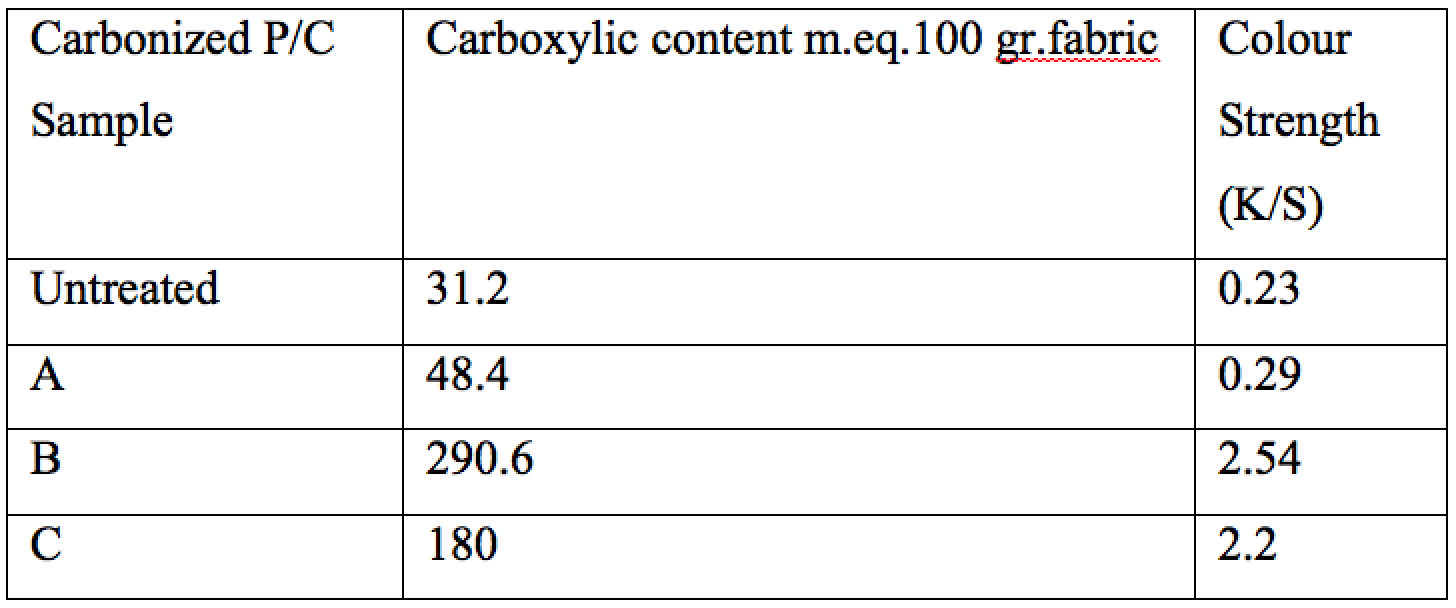
\includegraphics[width=0.7\textwidth]{1}
\end{center}

Appendix 2
\begin{center}
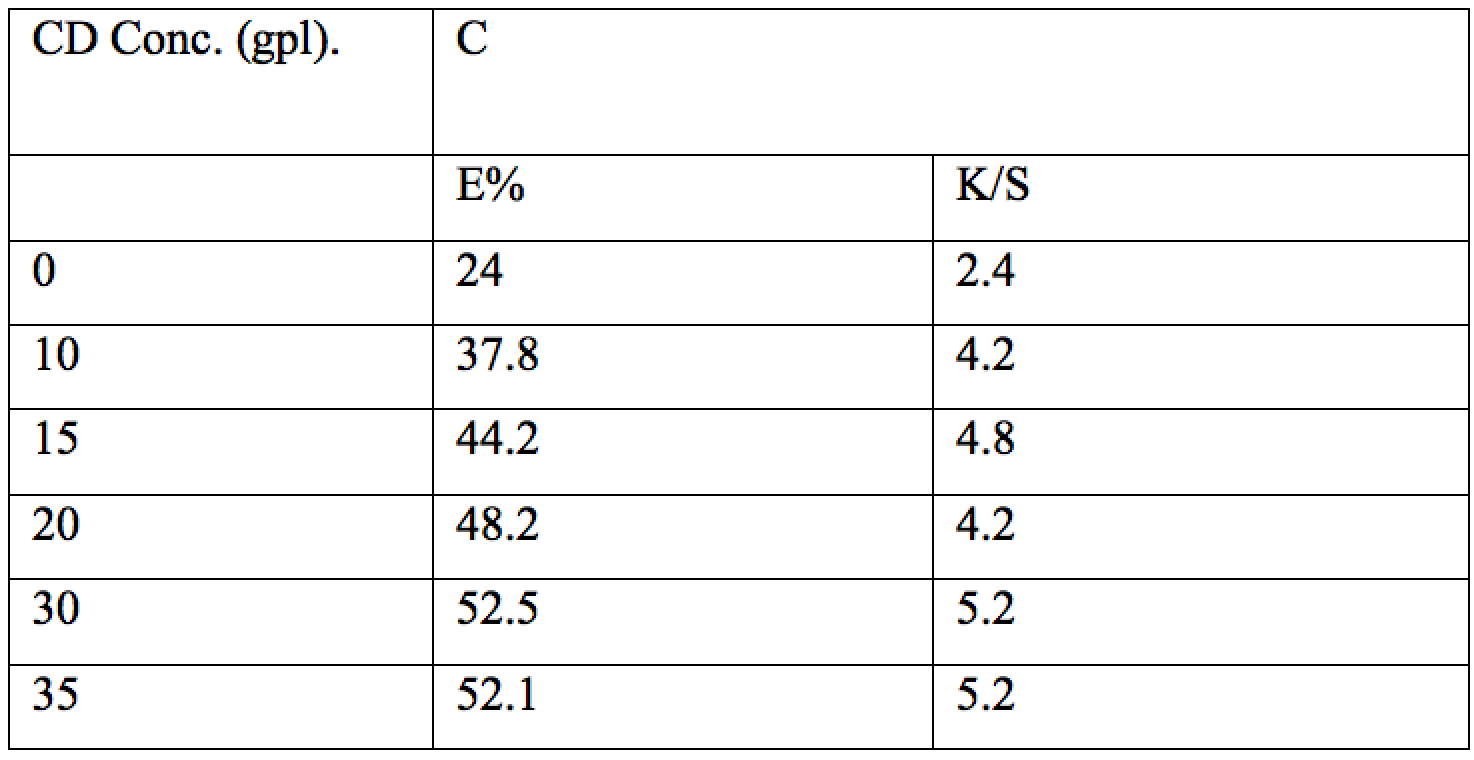
\includegraphics[width=0.9\textwidth]{2}
\end{center}

Appendix 3

\begin{center}
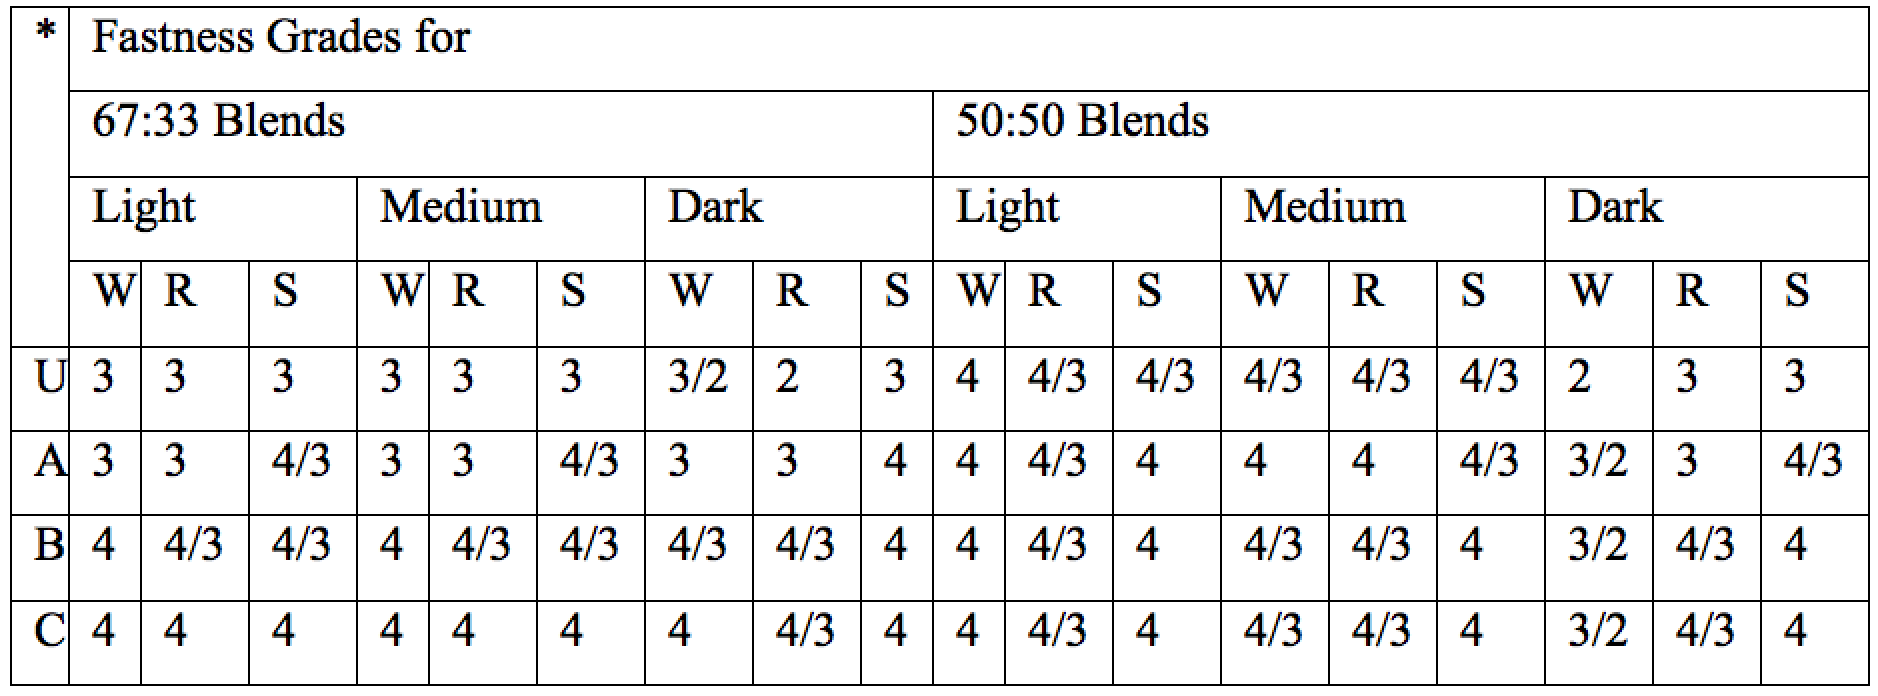
\includegraphics[width=0.9\textwidth]{3}
\end{center}

Appendix 4

\begin{center}
\begin{tabular}{ | c | c |}
\hline
Samples & Moisture Regain (\%) \\ \hline
Untreated & .42 \\ \hline
A & 0.96 \\ \hline
B & 1.33 \\ \hline
C & 1.52 \\ \hline
D & 1.71 \\ \hline
\end{tabular}
\end{center}

Appendix 5

\begin{center}
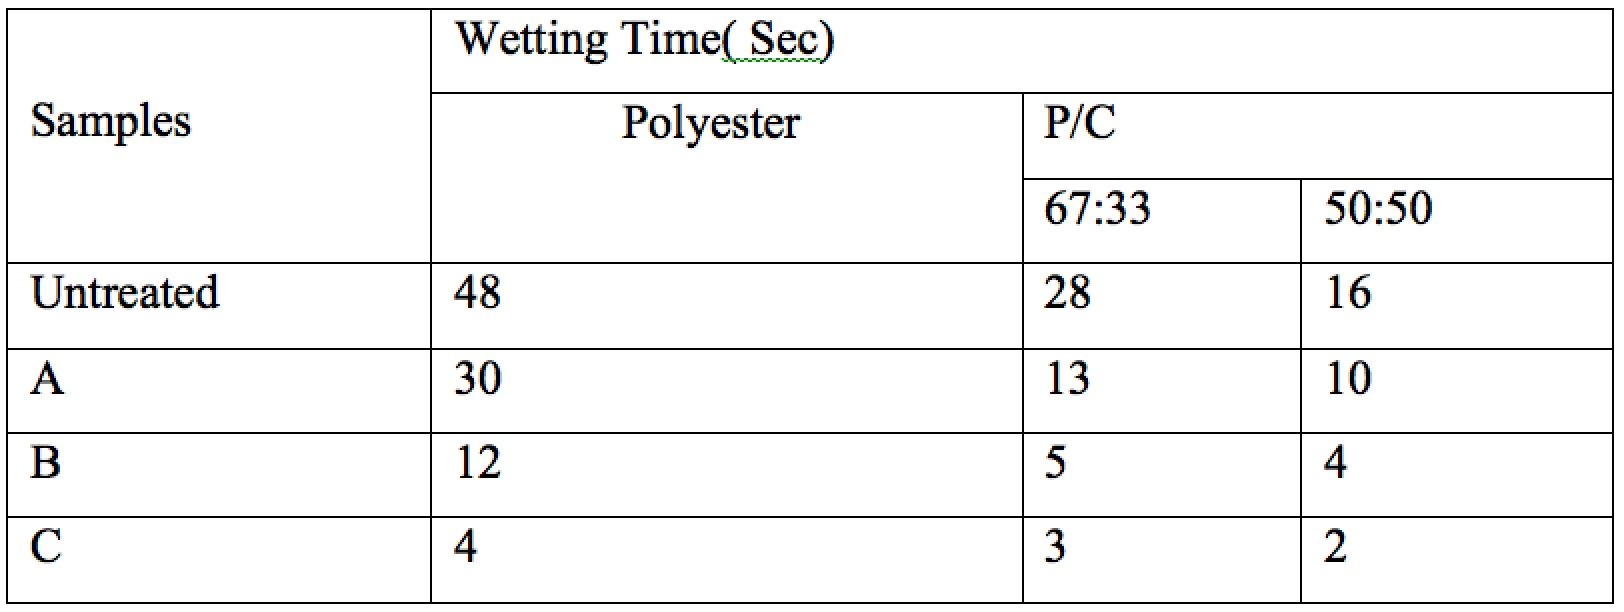
\includegraphics[width=0.9\textwidth]{5}
\end{center}

Appendix 6

\begin{center}
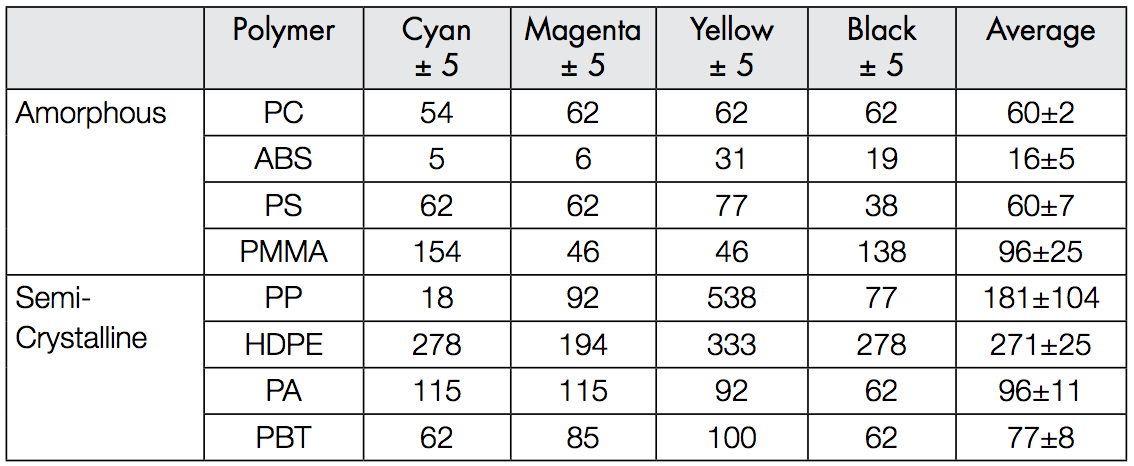
\includegraphics[width=0.9\textwidth]{6}
\end{center}

\begin{workscited}

\bibent
Kothari, Vasant.  ``Sublimation Print for Textile Material."  \textit{Screen Print India}.  July 2011.

\bibent
Periyasamy, Aravin.  ``Economical Dyeing of Polyester/Cotton Blends with Multifunctional Property By Using Cyclodextrins."  \textit{Screen Print India}.  July 2011.

\bibent
Bemska, Jadwiga. ``Surface Modification of Cotton Fabrics for Sublimation Printing." \textit{Autex Research Journal}. September 2013.

\bibent
Zschimmer \& Schwarz. Polappret PU-S. Koblenz: Zschimmer \& Schwarz. Web. February 2014

\bibent
Mao, Ya-Hong. ``Carrier Dyeing of Polyphenylene Sulphide Fabric With Disperse Dye." \textit{Coloration Technology}. November 2012.

\bibent
Lamb, Jimmy. ``How To Sublimate Apparel." \textit{Impressions}. March 2014

\bibent
Abdel-Latif, E. ``Synthesis of 5-arylazo-2-(arylidenehydrazino)-thiazole disperse dyes for dyeing polyester fibres." \textit{Pigment and Resin Technology}. January 2009.

\bibent
Annen, O. ``Replacement of Disperse Anthraquinone Dyes." \textit{Coloration Technology}. March 2008.

\bibent
Gaffer, Hatem. ``New Azo Disperse Dyes Containing Cyclohexanone Ring for Dyeing Polyester and Nylon Fabrics." \textit{Macedonian Journal of Chemistry and Chemical Engineering}. January 2010.

\bibent
King, Kerry. ``Emerging Technologies for Digital Textile Printing." \textit{AATCC Review}. August 2009.

\bibent
Histand, Matt. ``Dye Sublimation." \textit{Wearables} 12 (2008): 10. Business Source Complete. Web. Accessed 19 April 2014.

\bibent
History of Dye Sublimation. JVC Knowledge Base. Accessed 23 April 2014. <http://www3.jvckenwood.com/english/di/technology/history.html>.

\bibent
Mandol, R. ``Conventional Vs. Direct Dye Sublimation." Screen Printing 99.5 (2009): 12-3. SCOPUS. Web. 23 Apr. 2014.

\bibent
Kimbrough, Tonia Cook. ``Sublime Sublimating Technology." \textit{Wearables} 17.4 (2013): 36. Business Source Complete. Web. 20 April 2014.

\bibent
Allen, Art. ``Sublimation Printing - Minimizing Environmental Impact." AATCC Symposium Papers (2008): 134. Publisher Provided Full Text Searching File. Web. 21 Apr. 2014.


\end{workscited}
\end{mla}
\end{document}
